\documentclass{article}
\usepackage{graphicx} % Required for inserting images
\usepackage[utf8]{inputenc}
\usepackage{polski}
\usepackage[dvipsnames]{xcolor}
\usepackage{indentfirst}
\usepackage{multicol}
\usepackage{geometry}
\usepackage{titlesec}
\usepackage[colorlinks=true, linkcolor=gray, urlcolor=blue, citecolor=green]{hyperref}
\usepackage{makecell}
\usepackage{float}
\usepackage[polish]{babel}
\usepackage[T1]{fontenc}
\usepackage[justification=centering]{caption}
\usepackage[utf8]{inputenc} 
\usepackage{subfig}


\usepackage{mwe} % for 'example-image'
\usepackage{newfloat}
\DeclareFloatingEnvironment{graph}
\addto\captionspolish{%
  \renewcommand{\graphname}{Wykres}%
  \renewcommand{\figurename}{Rysunek}%
  \renewcommand{\tablename}{Tabela}%
}


\begin{document}

\begin{titlepage}
    \begin{center}
        \vspace*{1cm}
            
        \Huge
        \textbf{Sprawozdanie z laboratorium 6}
            
        \vspace{0.5cm}
        \LARGE
        HART (WAGO)
            
        \vspace{1.5cm}
            
        \textbf{Łukasz Janusz\\Marek Generowicz}

        \normalsize      
        \textcolor{gray}{09.03.2025}
        \vfill
        \begin{figure}[hb]
            \centering
            
\includegraphics[width=0.5\textwidth]{media/Logo_AGH.jpg}
        \end{figure}   
    \end{center}
\end{titlepage}

\section{Wstęp}
Na laboratoriach należało zapoznać się z protokołem HART, zasadami komunikacji oraz praktycznymi aspektami wykorzystania go w przemyśle. W trakcie zajęć przeprowadzono ćwiczenia z wykorzystaniem sterownika \textit{WAGO 750-841} wyposażonym w dwukanałowy analogowy moduł wejścia, który pozwala na komunikację z urządzeniami HART. Elementem pomiarowym natomiast jest \textit{termopara typu K}, która została połączona z modułem WAGO za pomocą przetwornika temperatury \textit{TxIsoRail-HART}. 
\subsection{Protokół HART}
Protokół HART \textit{(High Addressable Remote Transducer)} jest standardem komunikacyjnym stosowanym w przemyśle, który pozwala na komunikację z urządzeniami pomiarowymi, takimi jak czujniki, przetworniki, zawory, itp. Protokół HART umożliwia przesyłanie danych cyfrowych i analogowych w jednym przewodzie. Komunikacja odbywa się za pomocą sygnałów modulowanych na sygnale prądu stałego, co pozwala na przesyłanie danych cyfrowych wraz z sygnałem analogowym. Protokół HART jest kompatybilny z większością urządzeń pomiarowych, co pozwala na łatwe wdrożenie w istniejących systemach. Urządzenia, które wykorzystują protokół HART, są podzielone na nadrzędne (np. sterowniki PLC) i podrzędne (np. czujniki).
\newpage
\section{Przebieg ćwiczenia}

\subsection{Konfiguracja PLC}
W pierwszej części zadania należało zaprogramować sterownik \textit{WAGO}. W tym celu należało skorzystać z aplikacji \textit{CoDeSys}. Ważne aby w nowo stworzonym projekcie ustawić \textit{Type od POU} na \textit{Program} a język programowania na \textit{FBD} ze względy na konieczność wykorzystania biblioteki do obsługi \textit{POU} napisanej w tym właśnie języku. Następnie należało dodać moduły wejścia i wyjścia w wirtualnym wnętrzu magistrali. Uzupełniona magistrala wyglądała jak na zdjęcie \ref{fig1}.

\vspace{1em}
\begin{figure}[ht]
    \centering
    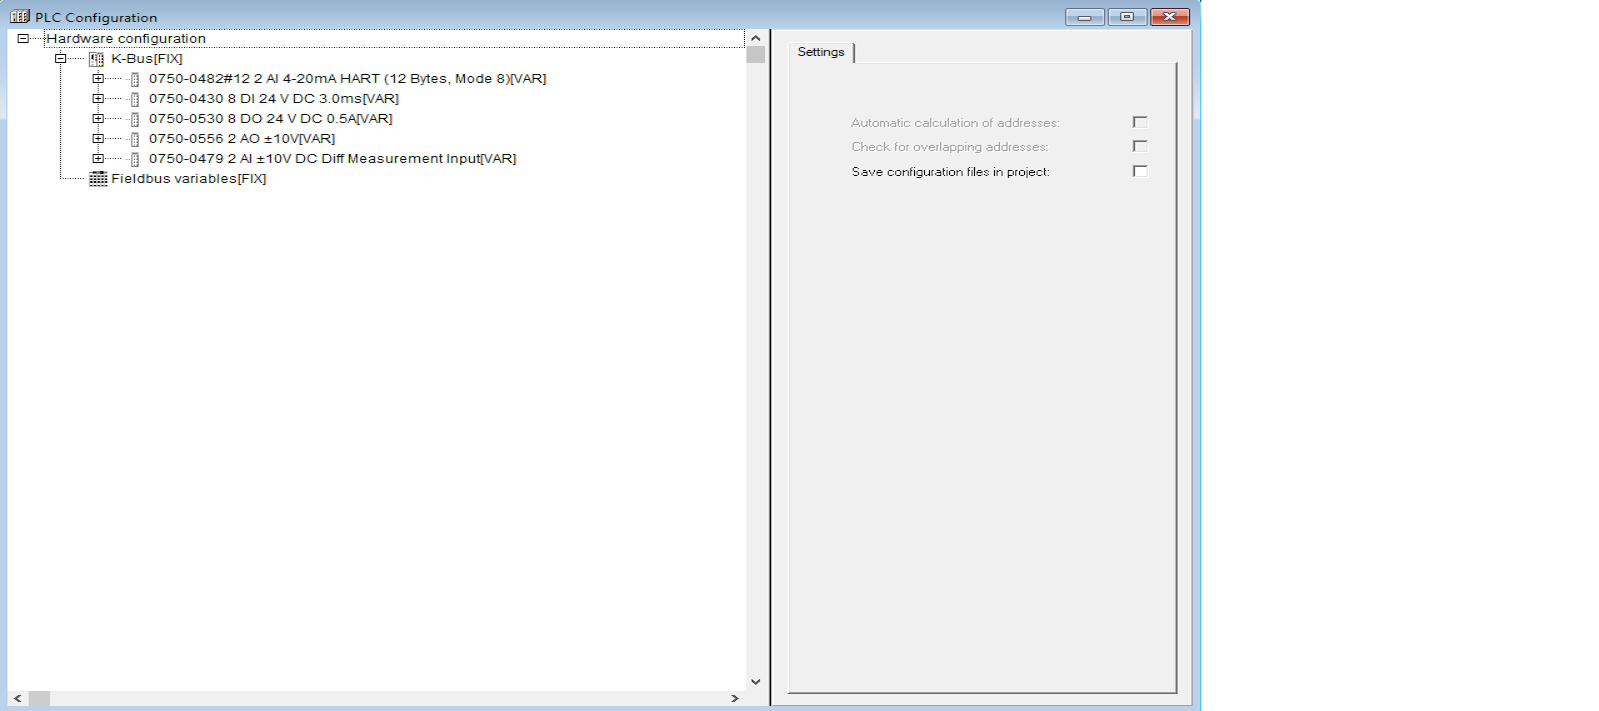
\includegraphics[width=1.3\linewidth]{media/6.png}
    \caption{Wnętrze magistrali w aplikacji \textit{CoDeSys}.}
    \label{fig1}
\end{figure}

Przed przystąpieniem do programowania należało skonfigurować parametry komunikacji oraz, w razie gdyby jej nie było, dodać bibliotekę do obsługi komunikacji HART \textit{WagoLibHART\_03.lib}
\newpage


\subsection{Program - HART\_INFO} \label{1a}
Po skonfigurowaniu PLC należało przejść do napisania kodu obsługującego moduł HART. Okno programu jest podzielone na dwie części, w górnej znajdują się zmienne używane w kodzie, a w dolnej znajduje się logika kodu. Zdjęcie \ref{fig2} przedstawia całość kodu napisanej na zajęciach aplikacji. Jak widać logika zależy od trzech bloków logicznych.

\vspace{1em}
\begin{figure}[ht]
    \centering
    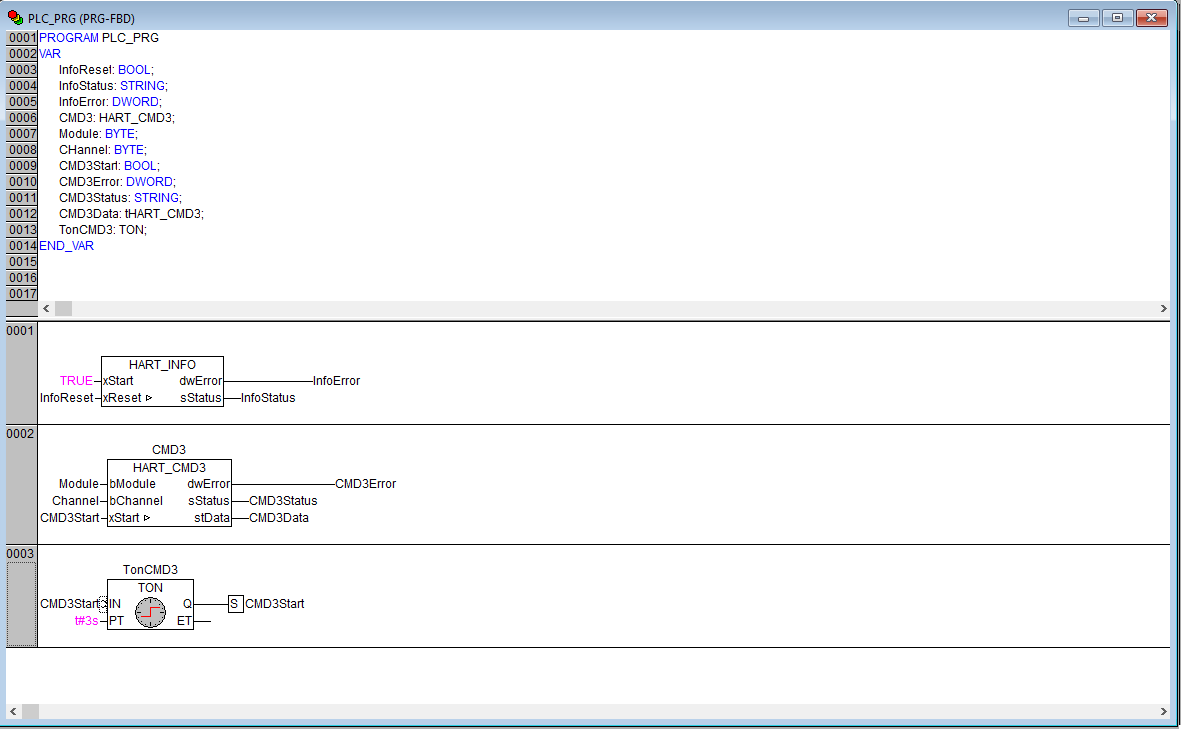
\includegraphics[width=1\linewidth]{media/4.png}
    \caption{Program obsługujący wejście analogowe modułu HART.}
    \label{fig2}
\end{figure}
\vspace{2em}

Pierwszy z nich \textit{HART\_INFO} służy do odczytu czy cały układ jest w stanie komunikować się z modułem HART. 

Drugi blok \textit{HART\_CMD3} za pomocą uniwersalnej komendy HART numer 3 służy do odczytu zmiennych w module HART.

Trzeci blok \textit{TON} jest zegarem, który pozwala na cykliczne wykonywanie logiki drugiego bloku, ponieważ blok ten jest uruchamiany rosnącym zboczem parametru \textit{CMD3Start}. Ważne jest aby wejście timera zanegować aby zegar działał zgodnie z tym co oczekujemy.
\newpage

Stworzenie takiego programu daje nam możliwość odczytu zmiennych z modułu HART, co jest niezbędne do dalszych działań. W trakcie uruchomiania programu wartości należało pamiętać aby ustawić wartości zmiennych \textit{Module} oraz \textit{Channel} na wartości 1. Wygląd uruchomionego programu przedstawia zdjęcie \ref{fig3}.

\vspace{1em}
\begin{figure}[ht]
    \centering
    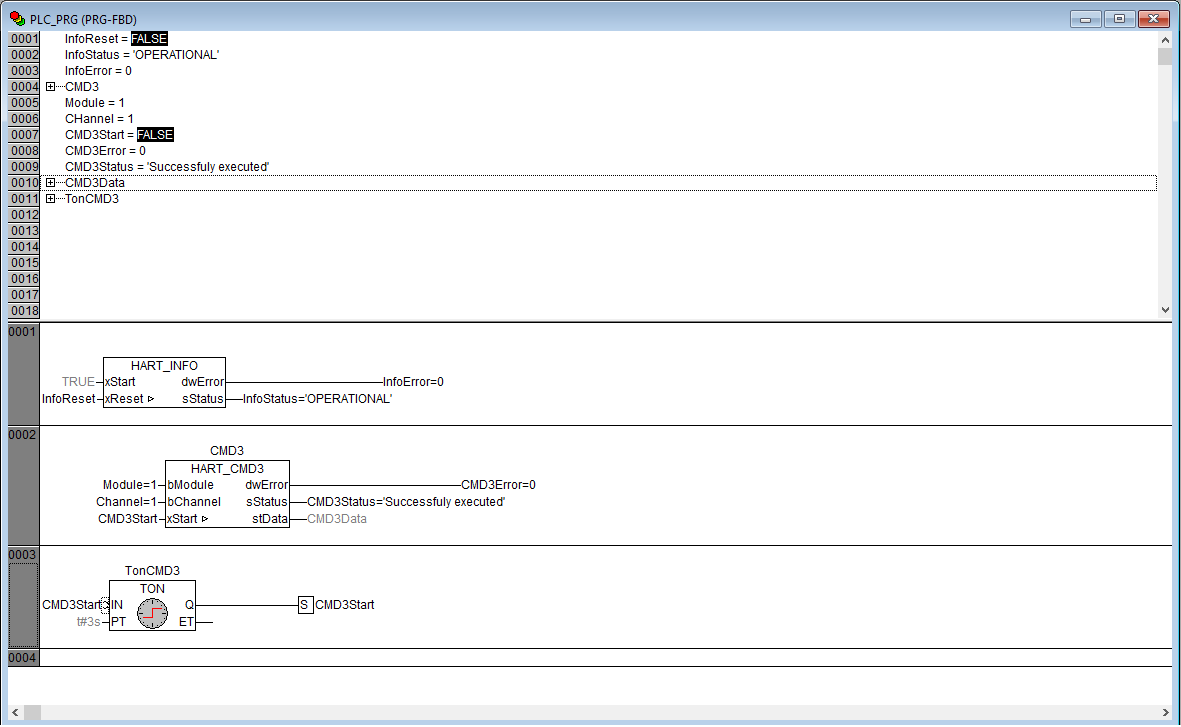
\includegraphics[width=1\linewidth]{media/3.png}
    \caption{Uruchomiony program do obsługi modułu HART.}
    \label{fig3}
\end{figure}

\newpage
\subsection{Program - odczyt zmiennych HART}
Po poprawnej konfiguracji oraz zaprogramowaniu sterownika, można przystąpić do odczytu zmiennych z modułu HART. W tym celu należy uruchomić program i ustawić poprawne wartości zmiennych \textit{Module} oraz \textit{Channel} na wartości 1. Po uruchomieniu programu, dzięki blokowi \textit{TON} program będzie cyklicznie co 6 sekund aktualizował dane, które moduł HART będzie otrzymywał od termopary typu K.

Aby odczytać wartości odebrane przez termoparę typu K oraz przekazane przez moduł HART, należy w części programu gdzie znajdują się parametry układu rozwinąć część \textit{CMD3Data}. Zdjęcie \ref{fig4} przedstawia jak wygląda odczyt zmiennych z modułu HART.


\vspace{1em}
\begin{figure}[ht]
    \centering
    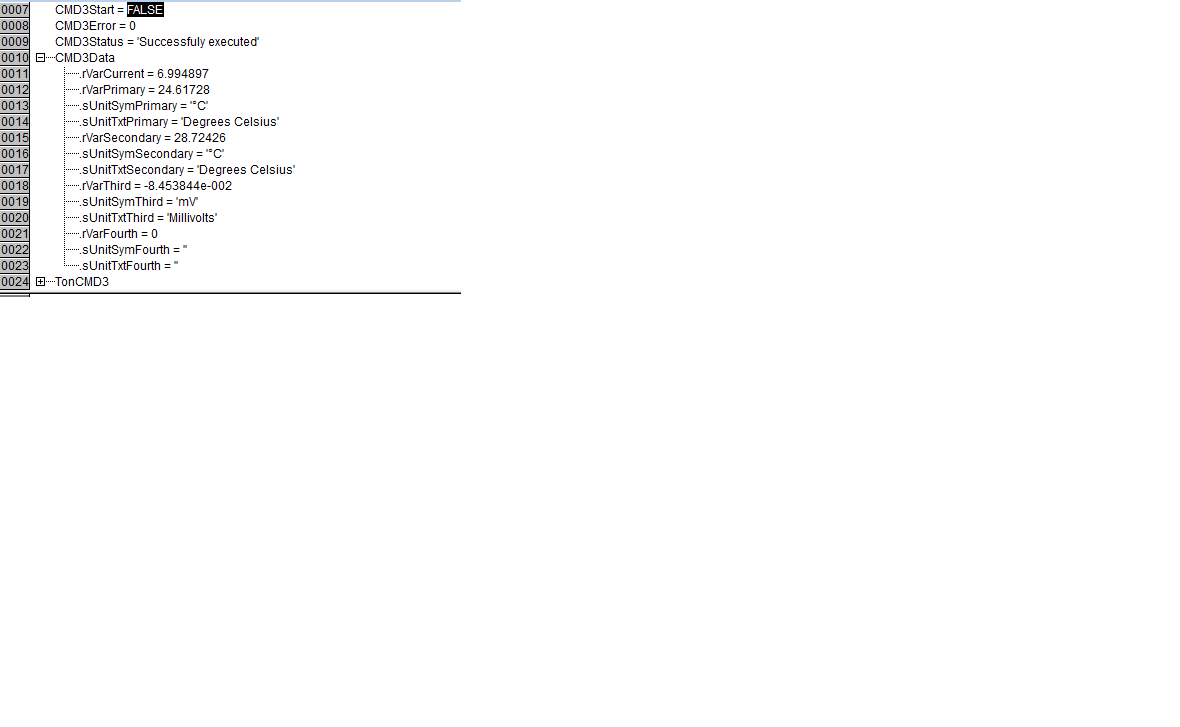
\includegraphics[width=1\linewidth]{media/1.png}
    \caption{Dane otrzymane z modułu HART.}
    \label{fig4}
\end{figure}

\newpage
\subsection{Dane HART}
W celu sprawdzenia ilości zmiennych dynamicznych należ skorzystać z  tabeli dostępnej w dokumentacji urządzenia. 
\begin{table}[H]
    \centering
    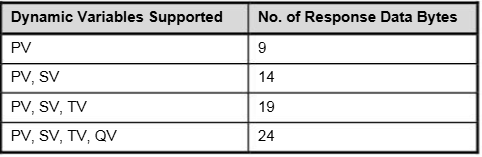
\includegraphics{media/Tabela_z_dokumentacji.png}
    \caption{Zależność między ilością zmiennych dynamicznych a długością tablicy CMD.abCmdData}
\end{table}
Aby tabela była użyteczna sprawdzamy wartość pola CMD3.bCmdDataCount, która w naszym przypadku wynosi 19.
\begin{figure}[H]
    \centering
    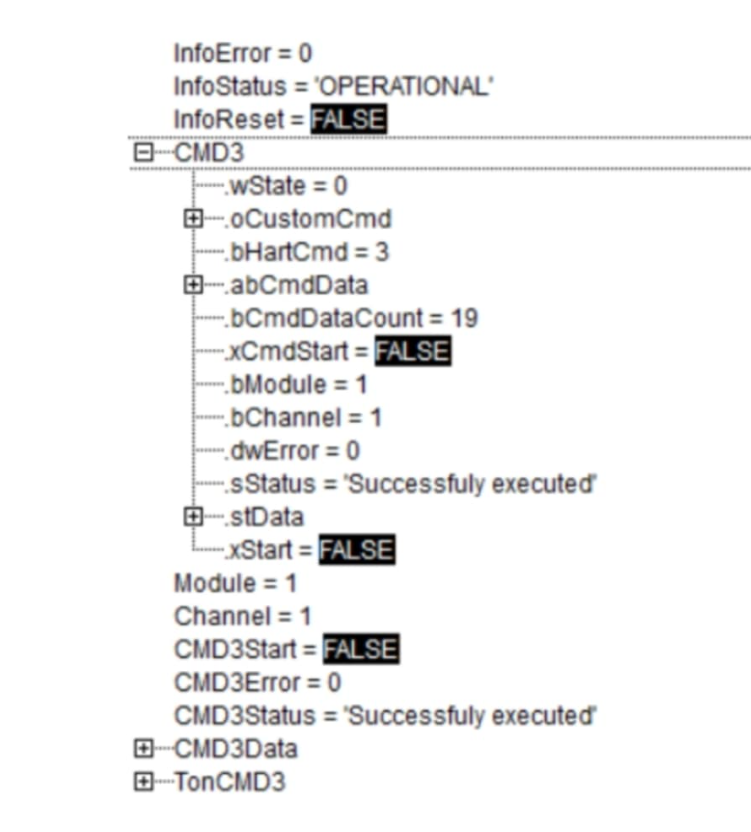
\includegraphics[width=0.5\linewidth]{media/19_ez.png}
    \caption{Wartość pola CMD3.bCmdDataCount}
\end{figure}
Dzięki temu wiadomo, że nasze urządzenie obsługuje dokładnie 3 zmienne dynamiczne.\\

Następnie należy sprawdzić jakie informacje są przekazywane w poszczególnych bitach oraz zdekodować i porównać znalezione wartości do danych widniejących w strukturze CMD3DATA. W celu sprawdzenia informacji o poszczególnych polach należy skorzystać z dokumentacji urządzenia.
\begin{table}[H]
    \centering
    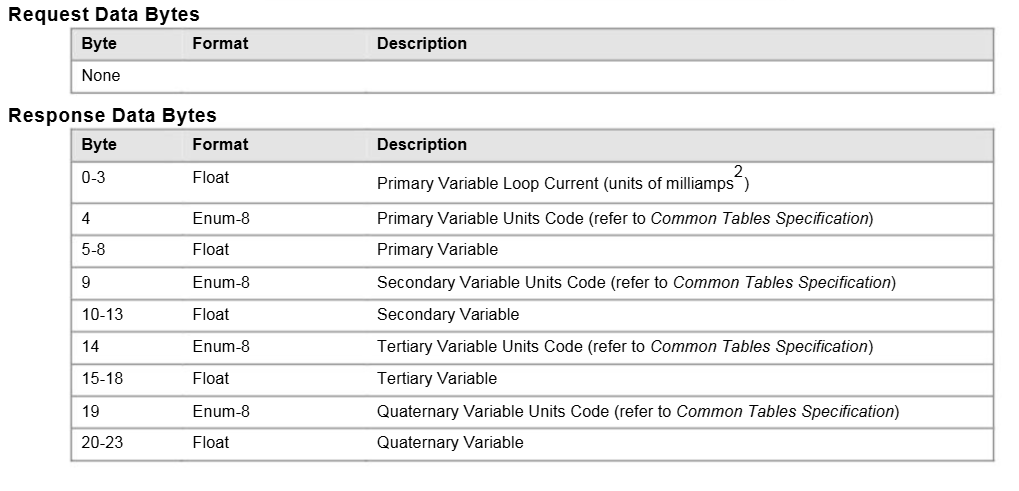
\includegraphics[width=0.9\linewidth]{media/Tabela_z_dokumentacji2.png}
    \caption{Znaczenie poszczególnych bitów w tabeli abCmdData}
\end{table}
W celu sprawdzenia wartości \textit{PV (Primary Value)} został użyty prosty program w języku C. 
\begin{figure}[H]
    \centering
    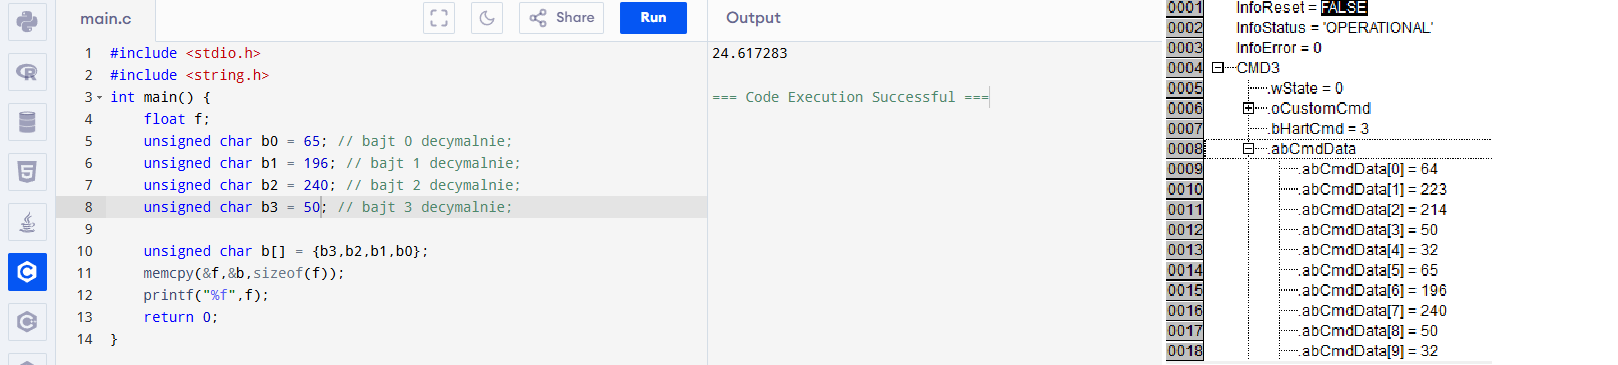
\includegraphics[width=0.8\linewidth]{media/8.png}
    \caption{Program w języku C do sprawdzenia wartości PV}
\end{figure}
Jak widać, jego odpowiedź jest zgodna (co do ilości wyśwetlanych miejsc po przecinku) z danymi wyświetlanymi w polu CMD3Data.rVarPrimary (Rysunek \ref{fig4}).
\\
Drugim sposobem sprawdzenia wartości \textit{PV} jest internetowy konwerter dostępny pod linkiem https://www.h-schmidt.net/FloatConverter/IEEE754.html. Po wprowadzeniu odczytanych wartości otrzymujemy identyczny wynik. 
\begin{figure}[H]
    \centering
    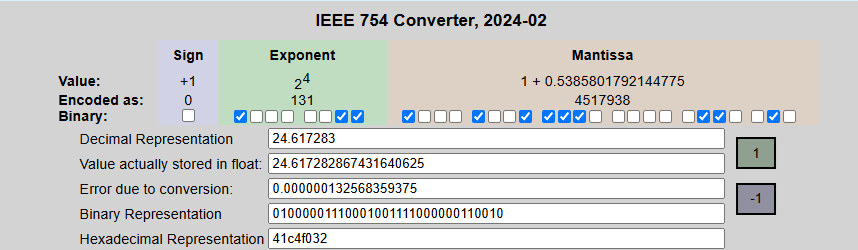
\includegraphics[width=0.8\linewidth]{media/konwersja2.png}
    \caption{Konwersja wartości binarnych na wartość PV}
\end{figure}

\newpage
\section{Podsumowanie}
Nauka programowania modułu HART jest bardzo przydatna ponieważ pozwala na komunikację z urządzeniami pomiarowymi w przemyśle ponieważ daje możliwość komunikacji dwukierunkowej nawet w niesprzyjających warunkach. W trakcie laboratoriów udało nam się zaprogramować sterownik \textit{WAGO 750-841}, odczytać dane z modułu HART oraz nauczyć się odczytywać "surowe" dane aby odczytać poszukiwane informacje. Dzięki temu zdobyliśmy praktyczną wiedzę na temat protokołu HART co umożliwi nam w przyszłości praktyczne wykorzystanie tej wiedzy w przemyśle.
\vspace{1em}
\begin{figure}[H]
    \centering
    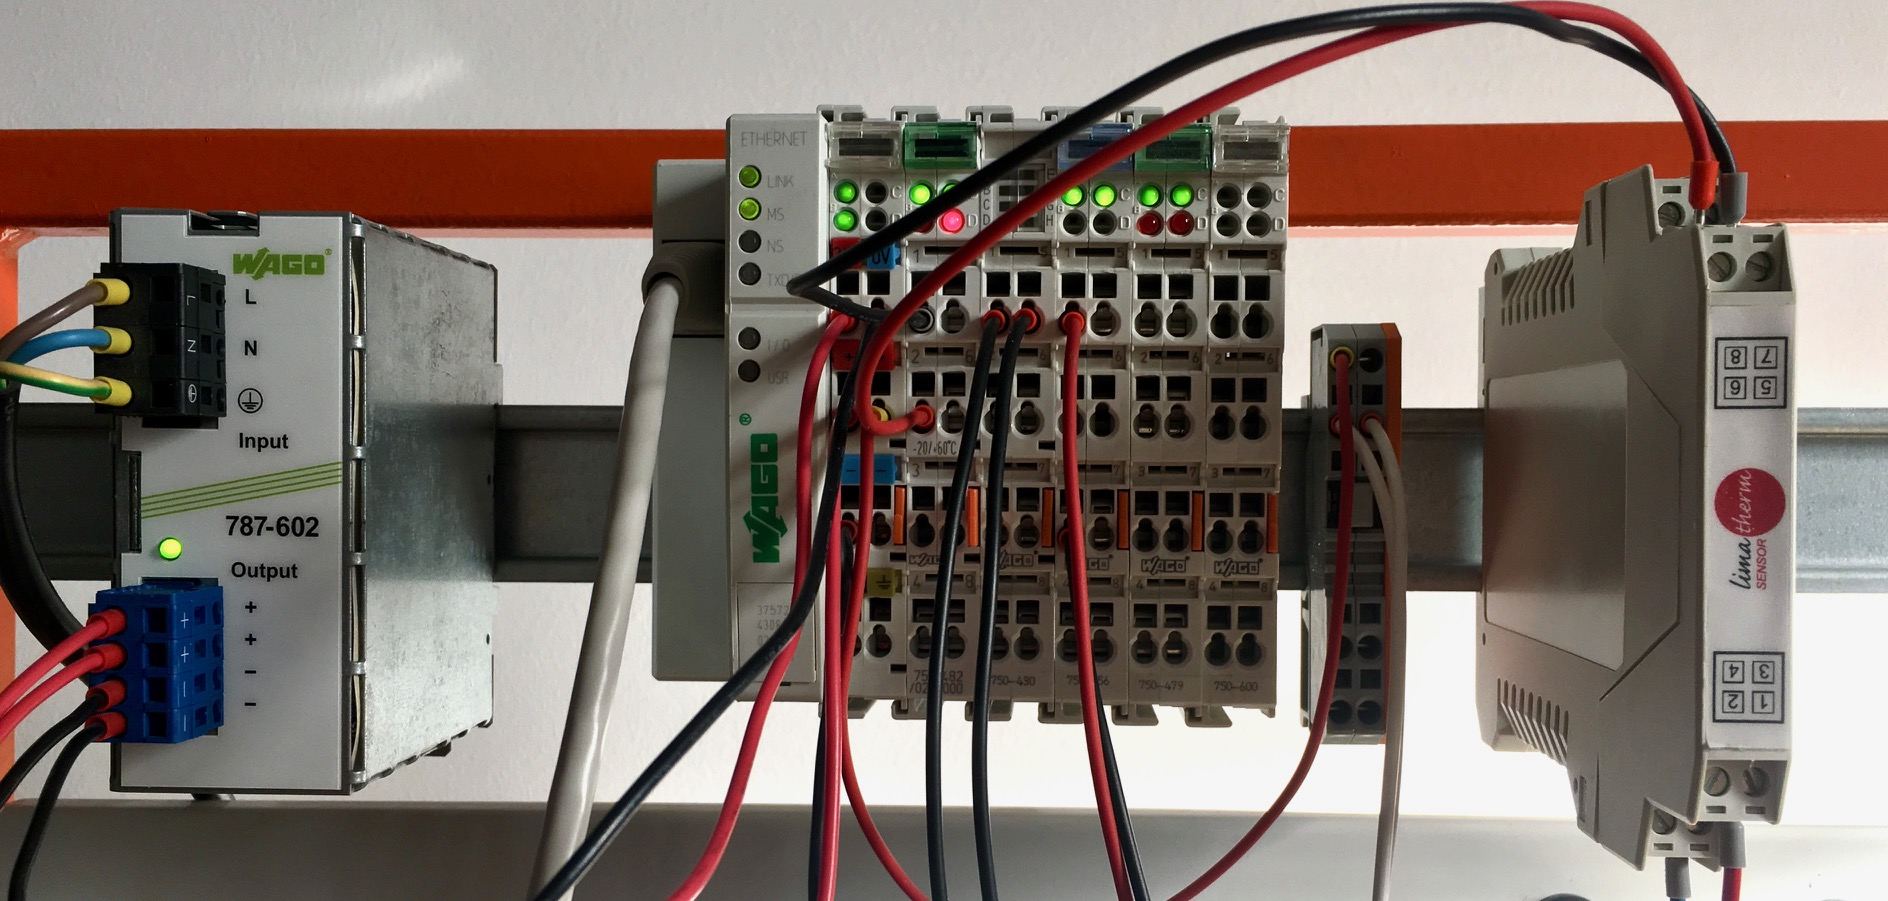
\includegraphics[width=1\linewidth]{media/HART.jpg}
    \caption{Wygląd modułu HART}
\end{figure}
\end{document}
